\chapter{Numerically stable transport over steep slopes}
\label{ch:cubicFit}

\section{Cubic fit transport scheme}

\begin{figure}
	\centering
	\documentclass[tikz]{standalone}
\newcommand{\vect}{\bm}
\newcommand{\Rearth}{R_e}
\newcommand{\lat}{\theta}
\newcommand{\lon}{\lambda}
\newcommand{\transpose}{\intercal}
\newcommand{\sign}{\mathrm{sgn}}
\newcommand{\unitlon}{\bm{\hat{\lon}}}
\newcommand{\unitlat}{\bm{\hat{\lat}}}
\newcommand{\unitk}{\bm{\hat{k}}}
\newcommand{\unitradius}{\bm{\hat{r}}}
\newcommand{\Mag}[1]{\left\lvert #1 \right\rvert}

\begin{document}
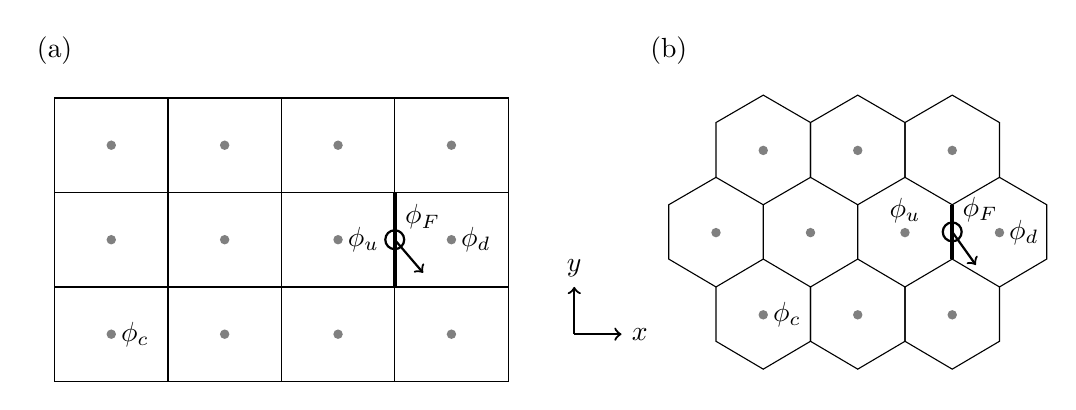
\begin{tikzpicture}[
  scale=0.6,
  cpnt/.style={fill=gray},
]

\begin{scope}[shift={(11,0)}]
	\draw [thick, ->] (0,1) -- (0,2) node [at end, anchor=south] {$y$};
	\draw [thick, ->] (0,1) -- (1,1) node [at end, anchor=west] {$x$};
\end{scope}

\node [above] at (0,6.5) {(a)};
\draw (0,0) rectangle (9.6,6);
\draw (0,2) -- (9.6,2);
\draw (0,4) -- (9.6,4);
\draw (0,0) -- (0,6);
\draw (2.4,0) -- (2.4,6);
\draw (4.8,0) -- (4.8,6);
\draw (7.2,0) -- (7.2,6);

\draw [ultra thick] (7.2,2) -- (7.2,4);
\draw [thick] (7.2,3) circle [radius=0.2] node [anchor=south west] {$\phi_F$};
\draw [thick, ->] (7.2,3) -- (7.8,2.3) node [anchor=west] {$\uf$};

\path [cpnt] (1.2,1) circle [radius=0.1] node [right] {$\phi_c$};
\path [cpnt] (1.2,3) circle [radius=0.1];
\path [cpnt] (1.2,5) circle [radius=0.1];

\path [cpnt] (3.6,1) circle [radius=0.1];
\path [cpnt] (3.6,3) circle [radius=0.1];
\path [cpnt] (3.6,5) circle [radius=0.1];

\path [cpnt] (6.0,1) circle [radius=0.1];
\path [cpnt] (6.0,3) circle [radius=0.1] node [right] {$\phi_u$};
\path [cpnt] (6.0,5) circle [radius=0.1];

\path [cpnt] (8.4,1) circle [radius=0.1];
\path [cpnt] (8.4,3) circle [radius=0.1] node [right] {$\phi_d$};
\path [cpnt] (8.4,5) circle [radius=0.1];

\begin{scope}[shift={(13,2)}]
	\node [above] at (0,4.5) {(b)};

	\draw (1,0) -- (0,0.59) -- (0,1.74) -- (1,2.32) -- (2,1.74) -- (2,0.59) -- (1,0); \path [cpnt] (1,1.15) circle [radius=0.1];
	\draw (2,1.74) -- (3,2.32) -- (4,1.74) -- (4,0.59) -- (3,0) -- (2,0.59); \path [cpnt] (3,1.15) circle [radius=0.1];
	\draw (4,1.74) -- (5,2.32) -- (6,1.74) -- (6,0.59) -- (5,0) -- (4,0.59); \path [cpnt] (5,1.15) circle [radius=0.1] node [above] {$\phi_u$};
	\draw (6,1.74) -- (7,2.32) -- (8,1.74) -- (8,0.59) -- (7,0) -- (6,0.59); \path [cpnt] (7,1.15) circle [radius=0.1] node [right] {$\phi_d$};

	\begin{scope}[shift={(1,-1.74)}]\draw (2,1.74) --(2,0.59) -- (1,0) -- (0,0.59) -- (0,1.74); \path [cpnt] (1,1.15) circle [radius=0.1] node [right] {$\phi_c$};\end{scope}
	\begin{scope}[shift={(3,-1.74)}]\draw (2,1.74) --(2,0.59) -- (1,0) -- (0,0.59) -- (0,1.74); \path [cpnt] (1,1.15) circle [radius=0.1];\end{scope}
	\begin{scope}[shift={(5,-1.74)}]\draw (2,1.74) --(2,0.59) -- (1,0) -- (0,0.59) -- (0,1.74); \path [cpnt] (1,1.15) circle [radius=0.1];\end{scope}

	\begin{scope}[shift={(1,1.74)}]\draw (0,0.59) -- (0,1.74) -- (1,2.32) -- (2,1.74) -- (2,0.59); \path [cpnt] (1,1.15) circle [radius=0.1];\end{scope}
	\begin{scope}[shift={(3,1.74)}]\draw (0,0.59) -- (0,1.74) -- (1,2.32) -- (2,1.74) -- (2,0.59); \path [cpnt] (1,1.15) circle [radius=0.1];\end{scope}
	\begin{scope}[shift={(5,1.74)}]\draw (0,0.59) -- (0,1.74) -- (1,2.32) -- (2,1.74) -- (2,0.59); \path [cpnt] (1,1.15) circle [radius=0.1];\end{scope}

	\draw [ultra thick] (6,0.59) -- (6,1.74);
	\draw [thick] (6,1.165) circle [radius=0.2] node [anchor=south west] {$\phi_F$};
	\draw [thick, ->] (6,1.165) -- (6.5,0.465) node [anchor=west] {$\uf$};
\end{scope}

\end{tikzpicture}
\end{document}

	\caption{Upwind-biased stencils for faces far away from the boundaries of two-dimensional (a) rectangular and (b) hexagon meshes.  The stencil is used to fit a multidimensional polynomial to cell centre values, $\phi_c$, marked by grey circles, in order to approximate the value $\phi_F$ at the face centroid marked by an open circle.  $\phi_u$ and $\phi_d$ are the values at the centroids of the upwind and downwind cells neighbouring the target face, drawn with a heavy line.  The velocity vector $\uf$ is prescribed at face $f$ and determines the choice of stencil at each time-step.}
	\label{fig:cubicFit:interiorStencils}
\end{figure}

The cubicFit scheme approximates the value of the dependent variable at the face, $\phi_F$, using a least-squares fit over a stencil of surrounding known values.
To introduce the approximation method, we will consider how an approximate value is calculated for a face that is far away from the boundaries of a two-dimensional uniform rectangular mesh.
For any mesh, every interior face connects two adjacent cells.  The velocity direction at the face determines which of the two adjacent cells is the upwind cell.  Since the stencil is upwind-biased and asymmetric, two stencils must be constructed for every interior face, and the appropriate stencil is chosen depending on the velocity direction at each face for every time-step.

The upwind-biased stencil for a face $f$ is shown in figure~\ref{fig:cubicFit:interiorStencils}a.  The wind at the face, $\uf$, is blowing from the upwind cell $c_u$ to the downwind cell $c_d$.
To obtain an approximate value at $f$, a polynomial least-squares fit is calculated using the stencil values.
The stencil has \num{4} points in $x$ and \num{3} points in $y$, leading to a natural choice of polynomial that is cubic in $x$ and quadratic in $y$,
\begin{align}
	\phi = a_1 + a_2 x + a_3 y + a_4 x^2 + a_5 xy + a_6 y^2 + a_7 x^3 + a_8 x^2 y + a_9 x y^2 \label{eqn:cubicFit:fullPoly} \text{ .}
\end{align}
A least-squares approach is needed because the system of equations is overconstrained, with \num{12} stencil values but only \num{9} polynomial terms.  The stencil geometry is expressed in a local coordinate system with the face centroid as the origin so that the approximated value $\phi_F$ is equal to the constant coefficient $a_1$.
The stencil is upwind-biased to improve numerical stability, and the multidimensional cubic polynomial is chosen to improve accuracy in the direction of flow \citep{leonard1993}.

The remainder of this \TODO{subsection} generalises the approximation technique for arbitrary meshes and describes the methods for constructing stencils, performing a least-squares fit with a suitable polynomial, and ensuring numerical stability of the transport scheme.

\subsection{Stencil construction}
\label{sec:cubicFit:stencil}

For every interior face, two stencils are constructed, one for each of the possible upwind cells.
Stencils are not constructed for boundary faces because values of $\phi$ at boundaries are calculated from prescribed boundary conditions.
For a given interior face $f$ and upwind cell $c_u$, we find those faces that are connected to $c_u$ and `oppose' face $f$.  These are called the \textit{opposing faces}.
The opposing faces for face $f$ and upwind cell $c_u$ are determined as follows.
Defining $G$ to be the set of faces other than $f$ that border cell $c_u$, we calculate the `opposedness', $\Opp$, between faces $f$ and $g \in G$, defined as
\begin{align}
	\Opp(f, g) \equiv - \frac{\Sf \cdot \vect{S}_g}{\magSf^2} \label{eqn:cubicFit:opp}
\end{align}
where $\Sf$ and $\vect{S}_g$ are the surface area vectors pointing outward from cell $c_u$ for faces $f$ and $g$ respectively.
Using the fact that $\vect{a} \cdot \vect{b} = \Mag{\vect{a}}\:\Mag{\vect{b}} \cos(\theta)$ we can rewrite equation~\eqref{eqn:cubicFit:opp} as
\begin{align}
	\Opp(f, g) = - \frac{\Mag{\vect{S}_g}}{\magSf} \cos(\theta)
\end{align}
where $\theta$ is the angle between faces $f$ and $g$.  In this form, it can be seen that $\Opp$ is a measure of the relative area of $g$ and how closely it parallels face $f$.

The set of opposing faces, $\mathrm{OF}$, is a subset of $G$, comprising those faces with $\Opp \geq 0.5$, and the face with the maximum opposedness.  Expressed in set notation, this is
\begin{align}
	\mathrm{OF}(f,c_u) \equiv \{ g : \Opp(f, g) \geq 0.5 \} \cup \{ g : \max_{g\:\in\:G}(\Opp(f, g)) \} \text{ .}
\end{align}
On a rectangular mesh, there is always one opposing face $g$, and it is exactly parallel to the face $f$ such that $\Opp(f, g) = 1$.

Once the opposing faces have been determined, the set of internal and external cells must be found.  The \textit{internal cells} are those cells that are connected to the opposing faces.  Note that $c_u$ is always an internal cell.  The \textit{external cells} are those cells that share vertices with the internal cells.  Note that $c_d$ is always an external cell.  Finally, the \textit{stencil boundary faces} are boundary faces having Dirichlet boundary conditions\footnote{Boundary faces with Neumann boundary conditions would require extrapolated boundary values to be calculated.
This would create a feedback loop in which boundary values are extrapolated from interior values, then interior values are transported using stencils that include boundary values.  
We have not considered how such an extrapolation could be made consistent with the multidimensional polynomial reconstruction.
Hence, boundary faces with Neumann boundary conditions are excluded from the set of stencil boundary faces.} that share a vertex with the internal cells.
Having found these three sets, the stencil is constructed to comprise all internal cells, external cells and stencil boundary faces.

\begin{figure}
	\centering
	\documentclass[tikz]{standalone}
\newcommand{\iu}{{i\mkern1mu}}
\newcommand{\vect}{\mathbf}
\newcommand{\unitg}{\vect{\hat{g}}}
\newcommand{\unitn}{\vect{\hat{n}}}
\newcommand{\uf}{\vect{u}_f}
\newcommand{\Opp}{\mathrm{Opp}}
\newcommand{\Sf}{\vect{S}_f}
\newcommand{\Mag}[1]{\lvert #1 \rvert}
\newcommand{\magSf}{\Mag{\Sf}}
\newcommand{\area}{\mathcal{A}}
\newcommand{\vol}{\mathcal{V}}
\newcommand{\volave}[1]{\langle #1 \rangle_\vol}
\newcommand{\moment}{\mathfrak{m}}
\newcommand{\rhoexp}{\mathfrak{n}}

\usetikzlibrary{plotmarks}
\usetikzlibrary{patterns}
\begin{document}
\begin{tikzpicture}[
  scale=0.25,
  cpnt/.style={fill=black},
]
\fill [pattern=north east lines,pattern color=gray] (5,0) -- (6,4) -- (3,7) -- (5, 15) -- (7,19) -- (1,19) -- (1,0);
\node at (0,9.5) {\rotatebox{90}{Dirichlet boundary}};

\draw [white] (-1,-2.1) rectangle (-1,-2);
\draw [thick, ->] (-1,-1.5) -- (4,-1.5) node [midway, anchor=south] {$\vect{u}$};

\draw [thick, ->] (20.7,7.5) -- (19.7,10) node [at end, anchor=south] {$y$};
\draw [thick, ->] (20.7,7.5) -- (23.1,8.35) node [at end, anchor=north] {$x$};

\draw (10,5) -- (20,7) -- (18,12) -- (11,14);
\draw [densely dashed, ultra thick] (11,14) -- (7,8) -- (10,5);
\draw [ultra thick] (20,7) -- (18,12);
\draw [thick] (19,9.5) circle [radius=0.35] node [anchor=east] {$f$};
\path [cpnt] (13.3,9.5) circle [radius=0.4] node [anchor=west, black] {$c_u$};
\path [fill=gray] (21.7,9.5) circle [radius=0.4] node [anchor=west, black] {$c_d$};

% direct upwind cells
\draw (10,5) -- (6,4) -- (3,7) -- (7,8);
\path [cpnt] (6.5,6) circle [radius=0.4];

\draw (3,7) -- (5,15) -- (11,14);
\path [cpnt] (6.3,11) circle [radius=0.4];

\draw (20,7) -- (24,6) -- (25,13) -- (18,12);
\draw (20,7) -- (19,3) -- (25,2) -- (24,6);
\draw (19,3) -- (11,1) -- (10,5);
\draw (11,14) -- (12,18) -- (16,18) -- (18,12);
\draw (16,18) -- (21,19) -- (25,13);
\draw (5,15) -- (7,19) -- (12,18);
\draw (6,4) -- (5,0) -- (11,1);

% vertices
\node at (3,7) {\pgfuseplotmark{square*}};
\node at (5,15) {\pgfuseplotmark{square*}};
\node at (11,14) {\pgfuseplotmark{square*}};
\node at (18,12) {\pgfuseplotmark{square*}};
\node at (10,5) {\pgfuseplotmark{square*}};
\node at (20,7) {\pgfuseplotmark{square*}};
\node at (6,4) {\pgfuseplotmark{square*}};
\node at (7,8) {\pgfuseplotmark{square*}};
\node at (5.5,2) [scale=1.5,rotate=60] {\pgfuseplotmark{triangle*}};
\node at (6,17) [scale=1.5,rotate=60] {\pgfuseplotmark{triangle*}};
\node at (4,11) [scale=1.5,rotate=60] {\pgfuseplotmark{triangle*}};
\node at (4.5,5.5) [scale=1.5,rotate=60] {\pgfuseplotmark{triangle*}};
\end{tikzpicture}
\end{document}

%	\includegraphics{../fig-double-upwind-stencil/fig-double-upwind-stencil.pdf}
	%
	\caption{A fourteen-point, upwind-biased stencil for face $f$ connecting the pentagonal upwind cell, $c_u$, and the downwind cell $c_d$.  The dashed lines denote the two faces of cell $c_u$ that oppose $f$, and black circles mark the centroids of the internal cells that are connected to these two opposing faces.  The stencil is extended outwards by including cells that share vertices with the three internal cells, where black squares mark these vertices.  Four stencil boundary faces, marked by black triangles, are also included.
The local coordinate system $(x, y)$ has its origin at the centroid of face $f$, marked by an open circle, with $x$ normal to $f$ and $y$ perpendicular to $x$.}
	\label{fig:double-upwind-stencil}
\end{figure}

Figure~\ref{fig:double-upwind-stencil} illustrates a stencil construction for face $f$ connecting upwind cell $c_u$ and downwind cell $c_d$.  The two opposing faces are denoted by thick dashed lines and the centres of the three adjoining internal cells are marked by black circles.  The stencil is extended outwards by including the external cells that share vertices with the internal cells, where the vertices are marked by black squares.  A boundary at the far left has Dirichlet boundary conditions, and so the four stencil boundary faces are also included in the stencil, where the boundary face centres are marked by black triangles.  The resultant stencil contains fourteen points.

\subsection{Least-squares fit}
To approximate the value of $\phi$ at a face $f$, a least-squares fit is calculated from a stencil of surrounding known values.  First, we will show how a polynomial least-squares fit is calculated for a face on a rectangular mesh.  Second, we will make modifications to the least-squares fit that are necessary for numerical stability.  

For faces that are far away from the boundaries of a rectangular mesh, we fit the multidimensional polynomial given by equation~\eqref{eqn:cubicFit:fullPoly} that has nine unknown coefficients, $\vect{a} = a_1 \ldots a_9$, using the twelve cell centre values from the upwind-biased stencil, $\bm{\phi} = \phi_1 \ldots \phi_{12}$.  This yields a matrix equation
\begin{align}
	\begin{bmatrix}
		1 & x_1 & y_1 & x_1^2 & x_1 y_1 & y_1^2 & x_1^3 & x_1^2 y_1 & x_1 y_1^2 \\
		1 & x_2 & y_2 & x_2^2 & x_2 y_2 & y_2^2 & x_2^3 & x_2^2 y_2 & x_2 y_2^2 \\
		\vdots & \vdots & \vdots & \vdots & \vdots & \vdots & \vdots & \vdots & \vdots \\
		1 & x_{12} & y_{12} & x_{12}^2 & x_{12} y_{12} & y_{12}^2 & x_{12}^3 & x_{12}^2 y_{12} & x_{12} y_{12}^2 \\
	\end{bmatrix}
	\begin{bmatrix}
		a_1 \\
		a_2 \\
		\vdots \\
		a_9
	\end{bmatrix}
	=
	\begin{bmatrix}
		\phi_1 \\
		\phi_2 \\
		\vdots \\
		\phi_{12}
	\end{bmatrix}
\end{align}
which can be written as
\begin{align}
	\vect{B} \vect{a} = \bm{\phi} \label{eqn:cubicFit:unweightedLeastSquares} \text{ .}
\end{align}
The rectangular matrix $\vect{B}$ has one row for each cell in the stencil and one column for each term in the polynomial.  $\vect{B}$ is called the \textit{stencil matrix}, and it is constructed using only the mesh geometry.
A local coordinate system is established in which $x$ is normal to the face $f$ and $y$ is perpendicular to $x$.
The coordinates $(x_i, y_i)$ give the position of the centroid of the $i$th cell in the stencil.
A two-dimensional stencil is also used for the tests on spherical meshes in section~\ref{sec:cubicFit:deformationSphere}.  In these tests, cell centres are projected perpendicular to a tangent plane at the face centre.  Previous studies found that results were largely insensitive to the projection method \citep{skamarock-gassmann2011,lashley2002}.

The unknown coefficients $\vect{a}$ are calculated using the pseudo-inverse, $\vect{B}^+$, found by singular value decomposition,
\begin{align}
	\vect{a} = \vect{B}^+ \bm{\phi} \text{ .}
%
\intertext{Recall that the approximate value $\phi_F$ is equal to the constant coefficient $a_1$, which is a weighted mean of $\bm{\phi}$,} 
%
	a_1 = \begin{bmatrix}
		b_{1,1}^+ \\
		b_{1,2}^+ \\
		\vdots \\
		b_{1,12}^+
	\end{bmatrix}
	\cdot
	\begin{bmatrix}
		\phi_1 \\
		\phi_2 \\
		\vdots \\
		\phi_{12}
	\end{bmatrix} \label{eqn:cubicFit:weighted-sum}
\end{align}
where the weights $b_{1,1}^+ \ldots b_{1,12}^+$ are the elements of the first row of $\vect{B}^+$.
Note that the majority of the least-squares fit procedure depends on the mesh geometry only.  An implementation may precompute the pseudo-inverse for each stencil during model initialisation, and only the first row needs to be stored.  Since each face has two possible stencils depending on the orientation of the velocity relative to the face, the implementation stores two sets of weights for each face.
Knowledge of the values of $\bm{\phi}$ is only required to calculate the weighted mean given by equation~\eqref{eqn:cubicFit:weighted-sum}, which is evaluated once per face per time-stage.

In the least-squares fit presented above, all stencil values contributed equally to the polynomial fit.
It is necessary for numerical stability that the polynomial fits the cells connected to face $f$ more closely than other cells in the stencil, as shown by \citet{lashley2002,skamarock-menchaca2010}.
To achieve this, we allow each cell to make an unequal contribution to the least-squares fit.
We assign an integer \textit{multiplier} to each cell in the stencil, $\vect{m} = m_1 \ldots m_{12}$, and multiply equation~\eqref{eqn:cubicFit:unweightedLeastSquares} to obtain
\begin{align}
	\vect{\tilde{B}} \vect{a} = \vect{m} \cdot \bm{\phi}
\end{align}
where $\vect{\tilde{B}} = \vect{M} \vect{B}$ and $\vect{M} = \mathrm{diag}(\vect{m})$.  The constant coefficient $a_1$ is calculated from the pseudo-inverse, $\vect{\tilde{B}}^+$,
\begin{align}
	a_1 = \vect{\tilde{b}_1^+} \cdot \vect{m} \cdot \bm{\phi} \label{eqn:cubicFit:weightedPinv}
\end{align}
where $\vect{\tilde{b}_1^+} = \tilde{b}_{1,1}^+ \ldots \tilde{b}_{1,12}^+$ are the elements of the first row of $\vect{\tilde{B}}^+$.
Again, $a_1$ is a weighted mean of $\bm{\phi}$, where the weights are now $\vect{\tilde{b}_1^+} \cdot \vect{m}$.  Values for $\vect{m}$ are chosen so that the cells connected to face $f$ make a greater contribution to the least-squares fit, as discussed later in section~\ref{sec:cubicFit:stabilisation}.

For faces of a non-rectangular mesh, or faces that are near a boundary, the number of stencil points and number of polynomial terms may differ: a stencil will have one or more cells and, for two-dimensional meshes, its polynomial will have between one and nine terms.  Additionally, the polynomial cannot have more terms than its stencil has cells because this would lead to an underconstrained system of equations.  The procedure for choosing suitable polynomials is discussed next.

\subsection{Polynomial generation}
\label{sec:cubicFit:polyGen}

\begin{figure}
	\centering
	\documentclass[tikz]{standalone}
\newcommand{\iu}{{i\mkern1mu}}
\newcommand{\vect}{\mathbf}
\newcommand{\unitg}{\vect{\hat{g}}}
\newcommand{\unitn}{\vect{\hat{n}}}
\newcommand{\uf}{\vect{u}_f}
\newcommand{\Opp}{\mathrm{Opp}}
\newcommand{\Sf}{\vect{S}_f}
\newcommand{\Mag}[1]{\lvert #1 \rvert}
\newcommand{\magSf}{\Mag{\Sf}}
\newcommand{\area}{\mathcal{A}}
\newcommand{\vol}{\mathcal{V}}
\newcommand{\volave}[1]{\langle #1 \rangle_\vol}
\newcommand{\moment}{\mathfrak{m}}
\newcommand{\rhoexp}{\mathfrak{n}}

\usetikzlibrary{patterns}
\begin{document}
\begin{tikzpicture}[
  scale=0.65,
  cpnt/.style={fill=gray},
]

\node [above] at (0,6) {(a)};
\fill [pattern=north east lines,pattern color=gray] (0,-1) rectangle (9,0);
\node at (4.5,-1.5) {Lower boundary};
\draw (0,0) rectangle (9,4);
\draw (3,0) -- (3,4);
\draw (6,0) -- (6,4);
\draw (0,2) -- (9,2);

\draw [ultra thick] (3,2) -- (6,2);
\draw [thick] (4.5,2) circle [radius=0.2];

\path [cpnt] (1.5,1) circle [radius=0.1];
\path [cpnt] (4.5,1) circle [radius=0.1] node [right] {$\phi_u$};
\path [cpnt] (7.5,1) circle [radius=0.1];
\path [cpnt] (1.5,3) circle [radius=0.1];
\path [cpnt] (4.5,3) circle [radius=0.1] node [right] {$\phi_d$};
\path [cpnt] (7.5,3) circle [radius=0.1];
\draw [thick, ->] (4.5,2) -- (5,2.35) node [anchor=west] {$\uf$};

\draw [<->] (6,5) node [left] {$y$} -- (7,5) -- (7,6) node [above] {$x$};

\begin{scope}[shift={(10,0)}]
\node [above] at (0,6) {(b)};
\fill [pattern=north east lines,pattern color=gray] (0,-1) rectangle (9,0);
\node at (4.5,-1.5) {Lower boundary};
\draw (0,0) rectangle (9,6);
\draw (3,0) -- (3,6);
\draw (6,0) -- (6,6);
\draw (0,2) -- (9,2);
\draw (0,4) -- (9,4);

\draw [ultra thick] (3,4) -- (6,4);
\draw [thick] (4.5,4) circle [radius=0.2];

\path [cpnt] (1.5,1) circle [radius=0.1];
\path [cpnt] (4.5,1) circle [radius=0.1];
\path [cpnt] (7.5,1) circle [radius=0.1];
\path [cpnt] (1.5,3) circle [radius=0.1];
\path [cpnt] (4.5,3) circle [radius=0.1] node [right] {$\phi_u$};
\path [cpnt] (7.5,3) circle [radius=0.1];
\path [cpnt] (1.5,5) circle [radius=0.1];
\path [cpnt] (4.5,5) circle [radius=0.1] node [right] {$\phi_d$};
\path [cpnt] (7.5,5) circle [radius=0.1];
\draw [thick, ->] (4.5,4) -- (5,4.35) node [anchor=west] {$\uf$};

\draw [<->] (10,5) node [left] {$y$} -- (11,5) -- (11,6) node [above] {$x$};
\end{scope}

\end{tikzpicture}
\end{document}

	\caption{Upwind-biased stencils for faces near the lower boundary of a rectangular $x$--$z$ mesh, with (a) a $3 \times 2$ stencil for the face immediately adjacent to the lower boundary, and (b) a $3 \times 3$ stencil for the face immediately adjacent to the face in (a).  Each stencil belongs to the face marked by a thick line.  The local coordinate system is shown, having an $x$ direction normal to the face a $y$ direction tangent to the face.  For both stencils, attempting a least-squares fit using the nine-term polynomial in equation~\eqref{eqn:cubicFit:fullPoly} would result in an underconstrained problem.
	There is no normal flow at the lower boundary.}
	\label{fig:cubicFit:boundaryStencils}
\end{figure}

The majority of faces on a uniform two-dimensional mesh have stencils with more than nine cells.  For example, a rectangular mesh has 12 points (figure~\ref{fig:cubicFit:interiorStencils}a), and a hexagonal mesh has 10 points (figure~\ref{fig:cubicFit:interiorStencils}b).
In both cases, constructing a system of equations using the nine-term polynomial in equation~\eqref{eqn:cubicFit:fullPoly} leads to an overconstrained problem that can be solved using least-squares.
However, this is not true for faces near boundaries: stencils that have fewer than nine cells (figure~\ref{fig:cubicFit:boundaryStencils}a) would result in an underconstrained problem, and stencils that have exactly nine cells may lack sufficient information to constrain high-order terms.
For example, the stencil in figure~\ref{fig:cubicFit:boundaryStencils}b lacks sufficient information to fit the $x^3$ term.  In such cases, it becomes necessary to perform a least-squares fit using a polynomial with fewer terms.

For every stencil, we find a set of \textit{candidate polynomials} that do not result in an underconstrained problem.
In two dimensions, a candidate polynomial has some combination of between one and nine terms from equation~\eqref{eqn:cubicFit:fullPoly}.  There are two additional constraints that a candidate polynomial must satisfy.

First, high-order terms may be included in a candidate polynomial only if the lower-order terms are also included.
More precisely, let
\begin{align}
	M(x, y) = { x^i y^j : i,j \geq 0 \text{ and } i \leq 3 \text{ and } j \leq 2 \text{ and } i+j \leq 3}
\end{align}
be the set of all monomials of degree at most \num{3} in $x, y$.
A subset $S$ of $M(x,y)$ is ``dense'' if, whenever $x^a y^b$ is in $S$, then $x^i y^j$ is also in $S$ for all $0 \leq i \leq a$, $0 \leq j \leq b$.
For example, the polynomial $\phi = a_1 + a_2 x + a_3 y + a_4 xy + a_5 x^2 + a_6 x^2 y$ is a dense subset of $M(x,y)$, but $\phi = a_1 + a_2 x + a_3 y + a_4 x^2 y$ is not because $x^2 y$ can be included only if $xy$ and $x^2$ are also included.
In total there are 26 dense subsets of the two-dimensional polynomial in equation~\eqref{eqn:cubicFit:fullPoly}.

Second, a candidate polynomial must have a stencil matrix $\vect{B}$ that is full rank.  The matrix is considered full rank if its smallest singular value is greater than \num{1e-9}.
Using a polynomial with all nine terms and the stencil in figure~\ref{fig:cubicFit:boundaryStencils}b results in a rank-deficient matrix and so the nine-term polynomial is not a candidate polynomial.

The candidate polynomials are all the dense subsets of $M(x,y)$ that have a cardinality greater than one with a stencil matrix that is full rank.  The final stage of the cubicFit transport scheme selects a candidate polynomial and ensures that the least-squares fit is numerically stable.

\subsection{Stabilisation procedure}
\label{sec:cubicFit:stabilisation}
So far, we have constructed a stencil and found a set of candidate polynomials.  Applying a least-squares fit to any of these candidate polynomials avoids creating an underconstrained problem.  The final stage of the transport scheme chooses a suitable candidate polynomial and appropriate multipliers $\vect{m}$ so that the fit is numerically stable.

The approximated value $\phi_F$ is equal to $a_1$ which is calculated from equation~\eqref{eqn:cubicFit:weightedPinv}.  The value of $a_1$ is a weighted mean of $\bm{\phi}$ where $\vect{w} = \vect{\tilde{b}_1^+} \cdot \vect{m}$ are the weights.
If the cell centre values $\bm{\phi}$ are assumed to approximate a smooth field then we expect $\phi_F$ to be close to the values of $\phi_u$ and $\phi_d$, and expect $\phi_F$ to be insensitive to small changes in $\bm{\phi}$.
When the weights $\vect{w}$ have large magnitude then this is no longer true: $\phi_F$ becomes sensitive to small changes in $\bm{\phi}$ which can result in large, numerically unstable departures from the smooth field $\bm{\phi}$.

To avoid numerical instabilities, a simplified, one-dimensional von Neumann analysis was performed, presented in appendix A.  The analysis is used to impose three stability conditions on the weights $\vect{w}$,
\begin{subequations}
\label{eqn:cubicFit:stability}
\begin{align}
	0.5 \leq w_u \leq 1 \label{eqn:cubicFit:stabilityU} \\
	0 \leq w_d \leq 0.5 \label{eqn:cubicFit:stabilityD} \\
	w_u - w_d \geq \max_{p\:\in\:P}(|w_p|)
\end{align}
\end{subequations}
where $w_u$ and $w_d$ are the weights for the upwind and downwind cells respectively.  The \textit{peripheral points} $P$ are the cells in the stencil that are not the upwind or downwind cells, and $w_p$ is the weight for a given peripheral point $p$.
 The upwind, downwind and peripheral weights sum to one such that $w_u + w_d + \sum_{p \in P} w_p = 1$.

The stabilisation procedure comprises three steps.  In the first step, the set of candidate polynomials is sorted in preference order so that candidates with more terms are preferred over those with fewer terms.
If there are multiple candidates with the same number of terms, the minimum singular value of $\vect{B}$ is calculated for each candidate, and an ordering is imposed such that the candidate with the larger minimum singular value is preferred.  This ordering ensures that the preferred candidate is the highest-order polynomial with the most information content.\footnote{Note that singular values are used for two purposes: first, to test if the matrix $\vect{B}$ is full-rank and, second, to impose an ordering on candidates.
We have used the minimum singular value, $\sigma_\mathrm{min}(\vect{B})$, for both purposes.  Alternatively, we could use the condition number, $\mathrm{cond}(\vect{B})$, which is the ratio of smallest to largest singular value.
Experiments revealed that only the candidate ordering was sensitive to the choice of $\sigma_\mathrm{min}$ or $\mathrm{cond}$.
The most suitable choices of singular value calculations could be explored in future.}

In the second step, the most-preferred polynomial is taken from the list of candidates and the multipliers are assigned so that the upwind cell and downwind cell have multipliers $m_u = 2^{10}$ and $m_d = 2^{10}$ respectively, and all peripheral points have multipliers $m_p = 1$.  These multipliers are very similar to those used by \citet{lashley2002}, leading to a well-conditioned matrix $\vect{\tilde{B}}$ and a least-squares fit in which the polynomial passes almost exactly through the upwind and downwind cell centre values.

In the third step, we calculate the weights $\vect{w}$ and evaluate them against the stability conditions given in equation~\eqref{eqn:cubicFit:stability}.
If any condition is violated, the value of $m_d$ is halved and the conditions are evaluated with the new weights.  This step is repeated until the weights satisfy the stability conditions, or $m_d$ becomes smaller than one.  In practice, the conditions are satisified when $m_d$ is either small (between 1 and 4) or equal to $2^{10}$.  The upwind multiplier $m_u$ is fixed at $2^{10}$ and the peripheral multipliers $m_p$ are fixed at \num{1}.  If the conditions are still not satisfied, then we start again from the second step with the next polynomial in the candidate list. 

Finally, if no stable weights are found for any candidate polynomial, we revert to an upwind scheme such that $w_u = 1$ and all other weights are zero.
In our experiments we have not encountered any stencil for which this last resort is required.
Furthermore, our experiments show that the stabilisation procedure only modifies the least squares fit for stencils near boundaries and for stencils in distorted mesh regions.
For stencils in the interior of a uniform rectangular mesh, the least squares fit includes all terms in equation~\eqref{eqn:cubicFit:fullPoly} with $m_u = m_d = 2^{10}$.

\begin{figure}
	\centering
	\input{cubicFit/stabilisation}
	\caption{One-dimensional least-squares fits with a stencil of five points using (a) a cubic polynomial with multipliers $m_u = 1024$, $m_d = 1024$ and $m_p = 1$, (b) a quadratic polynomial with the same multipliers, and (c) a quadratic polynomial with multipliers $m_u = 1024$, $m_d = 1$ and $m_p = 1$.  Notice that the curves in (a) and (b) fit almost exactly through the upwind and downwind points immediately adjacent to the $y$-axis, but in (c) the curve fits almost exactly only through the upwind point immediately to the left of the $y$-axis.  The point data are labelled with their respective weights.
	Points that have failed one of the stability conditions in equation~\eqref{eqn:cubicFit:stability} are marked in red with italicised labels.  The upwind point is located at $(-1, 1.8)$ and the downwind point at $(0.62, 1.9)$, and the peripheral points are at $(-2.8, 2.4)$, $(-1.6, 2.7)$ and $(-1.2, 2.2)$.  The stabilisation procedure (section~\ref{sec:cubicFit:stabilisation}) calculates weights using only $x$ positions, and values of $\phi$ are included here for illustration only.}
	\label{fig:cubicFit:oscillatory1D}
\end{figure}

To illustrate the stabilisation procedure, figure~\ref{fig:cubicFit:oscillatory1D}a presents a one-dimensional example of a cubic polynomial fitted through five points, with the weight at each point printed beside it.
The stabilisation procedure only uses the $x$ positions of these points and does not use the values of $\phi$ themselves.  The $\phi$ values are included here for illustration only.
Hence, for a given set of $x$ positions, the same set of weights are chosen irrespective of the $\phi$ values.

For a one-dimensional cubic polynomial fit, the list of candidate polynomials in preference order is
\begin{align}
	\phi &= a_1 + a_2 x + a_3 x^2 + a_4 x^3 \label{eqn:cubicFit:cubicCandidate} \text{ ,} \\
	\phi &= a_1 + a_2 x + a_3 x^2 \label{eqn:cubicFit:quadCandidate} \text{ ,} \\
	\phi &= a_1 + a_2 x \text{ ,} \\
	\phi &= a_1 \text{ .}
\end{align}
We begin with the cubic equation~\eqref{eqn:cubicFit:cubicCandidate}.  The multipliers are chosen so that the polynomial passes almost exactly through the upwind and downwind points that are immediately to the left and right of the $y$-axis respectively.
The stability condition on the upwind point is violated because $w_u = 1.822 > 1$ (equation~\ref{eqn:cubicFit:stabilityU}).  Reducing the downwind multiplier does not help to satisfy the stability condition, so we start again with the quadratic equation~\eqref{eqn:cubicFit:quadCandidate}, and the new fit is presented in figure~\ref{fig:cubicFit:oscillatory1D}b.
Again, the multipliers are chosen to force the polynomial through the upwind and downwind points, but this violates the stability condition on the downwind point because $w_d = 0.502 > 0.5$ (equation~\ref{eqn:cubicFit:stabilityD}).  This time, however, stable weights are found by reducing $m_d$ to one (figure~\ref{fig:cubicFit:oscillatory1D}c) and these are the weights that will be used to approximate $\phi_F$, where the polynomial intercepts the $y$-axis.

\subsection{Future extension to three dimensions}
All the procedures used in the cubicFit scheme generalise to three dimensions.  The stencil construction procedure described in section~\ref{sec:cubicFit:stencil} creates a stencil with \num{12} cells for a face in the interior of a two-dimensional rectangular mesh.  In three dimensions, the same procedure creates a stencil with $3 \times 12 = 36$ cells.
A three-dimensional stencil has three times as many cells as its two-dimensional counterpart if the mesh has prismatic cells arranged in columns.  Hence, the computational cost during integration increases three-fold when moving from two dimensions to three dimensions.

To extend the least squares fit to three dimensions, the two-dimensional polynomial in equation~\eqref{eqn:cubicFit:fullPoly} is replaced with its three-dimensional counterpart,
\begin{multline}
	\phi = a_1 + a_2 x + a_3 y + a_4 z + a_5 x^2 + a_6 xy + a_7 y^2 + a_8 xz + a_9 yz + a_{10} z^2 + \\ a_{11} x^3 + a_{12} x^2 y + a_{13} x y^2 + a_{14} x^2 z + a_{15} x z^2 + a_{16} y z^2 + a_{17} y^2 z + a_{18} xyz \text{ .} \label{eqn:cubicFit:fullPoly3D}
\end{multline}
The procedure for generating candidate polynomials described in section~\ref{sec:cubicFit:polyGen} results in 26 dense subsets in two dimensions and 842 dense subsets in three dimensions.  Note that the combinatorial explosion of dense subsets in three dimensions does not increase the computational cost during integration.

The stabilisation procedure described in section~\ref{sec:cubicFit:stabilisation} requires further numerical experiments to verify that it is sufficient for three-dimensional flows and arbitrary polyhedral meshes.
An initial three-dimensional test with uniform flow and a uniform Cartesian mesh obtained a numerically stable result.
For stencils in the interior of the domain, the least squares fit includes all polynomial terms in equation~\eqref{eqn:cubicFit:fullPoly3D} with $m_u = m_d = 2^{10}$.
The stabilisation procedure does not modify the least squares fit for these stencils, but we have not explored the three-dimensional extension of cubicFit any further.

\section{Deformational flow on a sphere}
\label{sec:cubicFit:deformationSphere}

The tests presented so far have used flows that are mostly uniform on meshes that are based on rectangular cells.
To ensure that the cubicFit transport scheme is suitable for complex flows on a variety of meshes, we use a standard test of deformational flow on a spherical Earth, as specified by \citet{lauritzen2012}.  
Results are compared between linearUpwind and cubicFit schemes using hexagonal-icosahedral meshes and cubed-sphere meshes.
Hexagonal-icosahedral meshes are constructed by successive refinement of a regular icosahedron following the approach by \citet{thuburn2014,heikes-randall1995a,heikes-randall1995b} without any mesh twisting.
Cubed-sphere meshes are constructed using an equi-distant gnomic projection of a cube having a uniform Cartesian mesh on each panel \citep{staniforth-thuburn2012}.

Following appendix A9 in \citet{lauritzen2014}, the average equatorial spacing $\Delta \lambda$ is used as a measure of mesh spacing.  It is defined as
\begin{align}
	\Delta \lambda = \ang{360} \frac{\overline{\Delta x}}{2 \pi R_e}
\end{align}
where $\overline{\Delta x}$ is the mean distance between cell centres and $R_e = \SI{6.3712e6}{\meter}$ is the radius of the Earth.

The deformational flow test specified by \citet{lauritzen2012} comprised six elements:
\begin{enumerate}
\item a convergence test using a Gaussian-shaped tracer
\item a ``minimal'' resolution test using a cosine bell-shaped tracer
\item a test of filament preservation
\item a test using a ``rough'' slotted cylinder tracer
\item a test of correlation preservation between two tracers
\item a test using a divergent velocity field
\end{enumerate}
We assess the cubicFit scheme using the first two tests only.  We do not consider filament preservation, correlation preservation, or the transport of a ``rough'' slotted cylinder because no shape-preserving filter has yet been developed for the cubicFit scheme.  Stable results were obtained when testing the cubicFit scheme using a divergent velocity field, but no further analysis is made here.

The first deformational flow test uses an infinitely continuous initial tracer that is transported in a non-divergent, time-varying, rotational velocity field.
The velocity field deforms two Gaussian `hills' of tracer into thin vortical filaments.  Half-way through the integration the rotation reverses so that the filaments become circular hills once again.  The analytic solution at the end of integration is identical to the initial condition.
A rotational flow is superimposed on a time-invariant background flow in order to avoid error cancellation.
The non-divergent velocity field is defined by the streamfunction $\Psi$,
\begin{align}
	\Psi(\lambda, \theta, t) = \frac{10 R_e}{T} \sin^2 \left(\lambda'\right) \cos^2 \left(\theta\right) \cos \left( \frac{\pi t}{T} \right) - \frac{2 \pi R_e}{T} \sin\left(\theta\right)
\end{align}
where $\lambda$ is a longitude, $\theta$ is a latitude, $\lambda' = \lambda - 2 \pi t / T$, and $T = \num{12}$ days is the duration of integration.  The time-step is chosen such that the maximum Courant number is about 0.4.

The initial tracer density $\phi$ is defined as the sum of two Gaussian hills,
\begin{align}
	\phi = \phi_1(\lambda, \theta) + \phi_2(\lambda, \theta) \text{ .}
\end{align}
An individual hill $\phi_i$ is given by
\begin{align}
	\phi_i(\lambda, \theta) = \phi_0 \exp\left( -b \left( \frac{\Mag{\vect{x} - \vect{x}_i}}{R_e} \right)^2 \right)
\end{align}
where $\phi_0 = \SI{0.95}{\kilo\gram\per\meter\cubed}$ and $b = 5$.  The Cartesian position vector $\vect{x} = (x,y,z)$ is related to the spherical coordinates $(\lambda, \theta)$ by
\begin{align}
	(x,y,z) = (R_e \cos \theta \cos \lambda, R_e \cos \theta \sin \lambda, R_e \sin \theta) \label{eqn:cubicFit:spherical-cartesian} \text{ .}
\end{align}
The centre of hill $i$ is positioned at $\vect{x}_i$.  In spherical coordinates, two hills are centred at
\begin{align}
	(\lambda_1,\theta_1) &= (5 \pi /6, 0) \\
	(\lambda_2,\theta_2) &= (7 \pi /6, 0)
\end{align}

\begin{figure}
	\centering
	\begin{subfigure}{0.35\textwidth}
		\caption{$t = \SI{0}{\second}$}
		\label{fig:cubicFit:deformationSphere-evolution:initial}
		\includegraphics{deformationSphere-gaussians-hex-8-cubicFit/0/tracer.pdf}
	\end{subfigure}
	\begin{subfigure}{0.3\textwidth}
		\caption{$t = T/2$}
		\label{fig:cubicFit:deformationSphere-evolution:mid}
		\includegraphics{deformationSphere-gaussians-hex-8-cubicFit/518400/tracerW.pdf}
	\end{subfigure}
	\begin{subfigure}{0.3\textwidth}
		\caption{$t = T$}
		\label{fig:cubicFit:deformationSphere-evolution:final}
		\includegraphics{deformationSphere-gaussians-hex-8-cubicFit/1036800/tracerW.pdf}
	\end{subfigure}
%
	\vspace{0.5em} \\
	\includegraphics[height=5in,angle=270]{deformationSphere-gaussians-hex-8-cubicFit/deformationSphere-gaussiansInitialTracer-colorBar.eps}
%
	\caption{Tracer fields for the deformational flow test using initial Gaussian hills.  The tracer is deformed by the velocity field before the rotation reverses to return the tracer to its original distribution:
	(\subcaptionref{fig:cubicFit:deformationSphere-evolution:initial}) the initial tracer distribution at $t = \SI{0}{\second}$;
	(\subcaptionref{fig:cubicFit:deformationSphere-evolution:mid}) by $t=T/2$ the Gaussian hills are stretched into a thin S-shaped filament;
	(\subcaptionref{fig:cubicFit:deformationSphere-evolution:final}) at $t=T$ the tracer resembles the initial Gaussian hills except for some distortion and diffusion due to numerical errors.  Results were obtained with the cubicFit scheme on a hexagonal-icosahedral mesh with an average equatorial mesh spacing of $\Delta \lambda = \inputval{deformationSphere-mesh-hex-8/averageEquatorialSpacing}$.}
	\label{fig:cubicFit:deformationSphere-evolution}
\end{figure}

The results in figure~\ref{fig:cubicFit:deformationSphere-evolution} are obtained using the cubicFit scheme on a hexagonal-icosahedral mesh with $\Delta \lambda = \inputval{deformationSphere-mesh-hex-8/averageEquatorialSpacing}$.
The initial Gaussian hills are shown in figure~\ref{fig:cubicFit:deformationSphere-evolution:initial}.
At $t=T/2$ the tracer has been deformed into an S-shaped filament (figure~\ref{fig:cubicFit:deformationSphere-evolution:mid}).
By $t=T$ the tracer has almost returned to its original distribution except for some slight distortion and diffusion that are the result of numerical errors (figure~\ref{fig:cubicFit:deformationSphere-evolution:final}).

\begin{figure}
	\centering
	\input{cubicFit/deformationSphere/gaussiansConvergence}
	\caption{Numerical convergence of the deformational flow test on the sphere using initial Gaussian hills.  $\ell_2$ errors (equation~\ref{eqn:l2-error}) and $\ell_\infty$ errors (equation~\ref{eqn:linf-error}) are marked at mesh spacings between \inputval{deformationSphere-mesh-hex-4/averageEquatorialSpacing} and \inputval{deformationSphere-mesh-hex-9/averageEquatorialSpacing} using the linearUpwind scheme (dotted lines) and the cubicFit scheme (solid lines) on hexagonal-icosahedral meshes and cubed-sphere meshes.}
	\label{fig:cubicFit:deformationSphere-gaussian-convergence}
\end{figure}

To determine the order of convergence and relative accuracy of the linearUpwind and cubicFit schemes, the same test was performed at a variety of mesh spacings betweeen $\Delta \lambda = \inputval{deformationSphere-mesh-hex-4/averageEquatorialSpacing}$ and $\Delta \lambda = \inputval{deformationSphere-mesh-hex-9/averageEquatorialSpacing}$ on hexagonal-icosahedral meshes and cubed-sphere meshes.  The results are shown in figure~\ref{fig:cubicFit:deformationSphere-gaussian-convergence}.
The solution is slow to converge at coarse resolutions, and this behaviour agrees with the results from \citet{lauritzen2012}.  Both linearUpwind and cubicFit schemes achieve second-order accuracy at smaller mesh spacings. 
For any given mesh type and mesh spacing, the cubicFit scheme is more accurate than the linearUpwind scheme.
Results are more accurate using hexagonal-icosahedral meshes compared to cubed-sphere meshes.  It is not known whether the larger errors on cubed-sphere meshes are due to mesh non-uniformities at panel corners but there is no evidence of grid imprinting in the error fields (not shown).

A slightly more challenging variant of the same test is performed using a quasi-smooth tracer field defined as the sum of two cosine bells,
\begin{align}
	\phi =
	\begin{cases}
		b + c \phi_1(\lambda, \theta) & \quad \text{if $r_1 < r$,} \\
		b + c \phi_2(\lambda, \theta) & \quad \text{if $r_2 < r$,} \\
		b			      & \quad \text{otherwise.}
	\end{cases}
\end{align}
The velocity field is the same as before.  This test is used to determine the ``minimal'' resolution, $\Delta \lambda_m$, which is specified by \citet{lauritzen2012} as the coarsest mesh spacing for which $\ell_2 \approx 0.033$.

\begin{table}
	\robustify\itshape
	\centering
	\begin{tabular}{l l S[detect-weight, detect-shape, detect-mode, round-mode=off]}
\toprule
	Transport scheme & Mesh type & {Minimal resolution (\si{\degree})} \\
\midrule
	linearUpwind & Cubed-sphere & \itshape 0.15 \\
	\makecell{FARSIGHT, grid-point semi-Lagrangian \\ \quad\citep{white-dongarra2011}} & Cubed-sphere & 0.1875 \\
	linearUpwind & Hexagonal-icosahedral & \itshape 0.2 \\
	\makecell{SLFV-SL, swept-area scheme \\ \quad\citep{miura2007}} & Hexagonal-icosahedral & 0.25 \\
	cubicFit & Cubed-sphere & \itshape 0.25 \\
	cubicFit & Hexagonal-icosahedral & 0.3 \\
	\makecell{ICON-FFSL, swept-area scheme \\ \quad\citep{miura2007}} & Triangular-icosahedral & 0.42 \\
\bottomrule
\end{tabular}
%
	\caption{Minimal resolutions for the cubicFit and linearUpwind schemes in the test of deformational flow using cosine bells.  Italicised values have been extrapolated using the second-order convergence obtained at coarser mesh spacings.  For comparison with existing models, some results are also included for unlimited versions of the transport schemes from the intercomparison by \citet{lauritzen2014}.}
	\label{tab:deformationSphere:minimal-resolution}
\end{table}

The minimal resolution for the cubicFit scheme on a hexagonal-icosahedral mesh is about $\Delta \lambda_m = \ang[round-precision=1]{0.3}$.  Tests were not performed at mesh spacings finer than $\Delta \lambda = \inputval{deformationSphere-mesh-hex-9/averageEquatorialSpacing}$ but approximate minimal resolutions have been extrapolated from the second-order convergence that is found at fine mesh spacings.  These minimal resolutions are presented in table~\ref{tab:deformationSphere:minimal-resolution} along with a selection of transport schemes having similar minimal resolutions from the model intercomparison by \citet{lauritzen2014}.

The series of deformational flow tests presented here demonstrate that the cubicFit scheme is suitable for transport on spherical meshes based on quadrilaterals and hexagons.  The cubicFit scheme is largely insensitive to the mesh type, and results are more accurate compared to the linearUpwind scheme for a given mesh type and mesh spacing.  Neither scheme requires special treatment at the corners of cubed-sphere panels.



